\documentclass[tikz,border=10pt]{standalone}
\usepackage{tikz}
\usetikzlibrary{calc,patterns,decorations.pathmorphing,decorations.markings}

% Suppress the page number
\pagenumbering{gobble}

\begin{document}
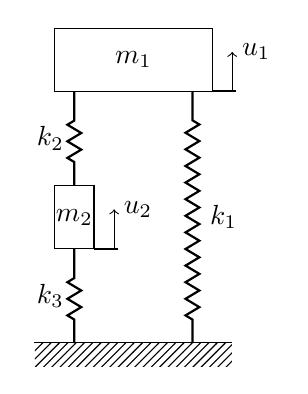
\begin{tikzpicture}

  \tikzstyle{spring}=[thick,decorate,decoration={zigzag,pre length=0.3cm,post length=0.3cm,segment length=6}]
\tikzstyle{damper}=[thick,decoration={markings,  
  mark connection node=dmp,
  mark=at position 0.5 with 
  {
    \node (dmp) [thick,inner sep=0pt,transform shape,rotate=-90,minimum width=15pt,minimum height=3pt,draw=none] {};
    \draw [thick] ($(dmp.north east)+(2pt,0)$) -- (dmp.south east) -- (dmp.south west) -- ($(dmp.north west)+(2pt,0)$);
    \draw [thick] ($(dmp.north)+(0,-5pt)$) -- ($(dmp.north)+(0,5pt)$);
  }
}, decorate]
\tikzstyle{ground}=[fill,pattern=north east lines,draw=none,minimum width=0.75cm,minimum height=0.3cm]



  % ====================
  % Parameters
  % ====================
  \def\massw{0.5cm}  % Width of the masses
  \def\massh{0.8}  % Height of the masses
  \def\spaceh{1.2} % Height of the springs/dampers
  \def\widthground{2.5cm}
  \def\dispw{0.3}  % Width of the dashed line for the displacement
  \def\disph{0.5}  % Height of the arrow for the displacements
  \def\bracs{0.05} % Brace spacing vertically
  \def\brach{-10pt} % Brace shift horizontaly
  % ====================


  % ====================
  % Ground
  % ====================
  \node (ground) [ground,anchor=south,minimum width=\widthground,yshift=-0.3cm] {};
  \draw (ground.north east) -- (ground.north west);

  \begin{scope}[shift={(0, 0)}]
    % Mass
    \draw[fill=white] (-2*\massw, \spaceh) rectangle (-1*\massw, \spaceh+\massh) node[pos=0.5]{$m_{2}$};

    % Spring, Damper, and Actuator
    \draw[spring] (-1.5*\massw, 0) -- (-1.5*\massw, \spaceh) node[midway, left=0.1]{$k_{3}$};
    
    % Displacements
    \draw[thick] (-1*\massw, \spaceh) -- ++(\dispw, 0);
    \draw[->] (-0.5*\massw+0.5*\dispw, \spaceh) -- ++(0, \disph) node[right]{$u_{2}$};
  \end{scope}

  \begin{scope}[shift={(0, \spaceh+\massh)}]
    % Mass
    \draw[fill=white] (-2*\massw, \spaceh) rectangle (2*\massw, \spaceh+\massh) node[pos=0.5]{$m_{1}$};

    % Spring, Damper, and Actuator
    \draw[spring] (-1.5*\massw, 0) -- (-1.5*\massw, \spaceh) node[midway, left=0.1]{$k_{2}$};
    
    % Spring, Damper, and Actuator
    \draw[spring] (1.5*\massw, -\spaceh-\massh) -- (1.5*\massw, \spaceh) node[midway, left=0.1,xshift=0.7cm]{$k_{1}$};

    % Displacements
    \draw[thick] (2.0*\massw, \spaceh) -- ++(\dispw, 0);
    \draw[->] (2.5*\massw+0.5*\dispw, \spaceh) -- ++(0, \disph) node[right]{$u_{1}$};

    % Legend
    % \draw[decorate, decoration={brace, amplitude=8pt}, xshift=\brach] %
    %   (-0.5*\massw, \bracs) -- (-0.5*\massw, \spaceh+\massh-\bracs) %
    %   node[midway,rotate=90,anchor=south,yshift=10pt]{};
  \end{scope}
\end{tikzpicture}

\end{document}
